%%%%%%%%%%%%%%%%%%%%%%
\chapter{Equilibrium interface dynamics}
\label{chap-int-dyn}
%%%%%%%%%%%%%%%%%%%%%%


In this chapter we will analyse the dynamics of statistical systems. The analysis will allow us to understand how phase transitions - in particular those who possess a phase separation - occur dynamically \cite{hohenberg_theory_1977}. The most famous example is the Ising model without any external field, its order parameter being the total magnetization. 

In the high temperature phase, the system is homogeneous and its total magnetization is zero. Below the critical temperature, when the order parameter is conserved (for example with a Kawasaki dynamic or Model B), the system will locally separate into two phases of opposite mean magnetization separated by and interface, this interface minimizing the surface energy between both phases.
When the order parameter is not conserved (for example Glauber dynamics or Model A), a spontaneous symmetry breaking will make one of the two phases take over the whole system. In a continuous phase transition where the critical point is reached from the disordered state to the ordered stated, the domain size, which is equal to the system's correlation length, diverges close to the critical temperature $T_C$. In a thermodynamical system, it becomes infinite, implying that the system takes an infinite amount of time to reach equilibrium : it's the critical slowing down. The process of domain growth is known as coarsening and phase ordering kinetics is the theory that has been developed to understand the phenomenon of coarsening\cite{bray_theory_1994}.  In Fig \ref{clusterization}, we show an example of coarsening in the Ising model with respect to time.

Furthermore, for systems with a conserved order parameter which separate into two phases, the two phases will be separated by an interface. This interface will be characterised by a surface tension, its average position will be fixed but it will exhibit fluctuations. Later we will see how model of phase ordering kinetics and be used to determine the static and dynamical properties of interfaces between two coexisting phases. 

\begin{figure}[t]
    \centering
    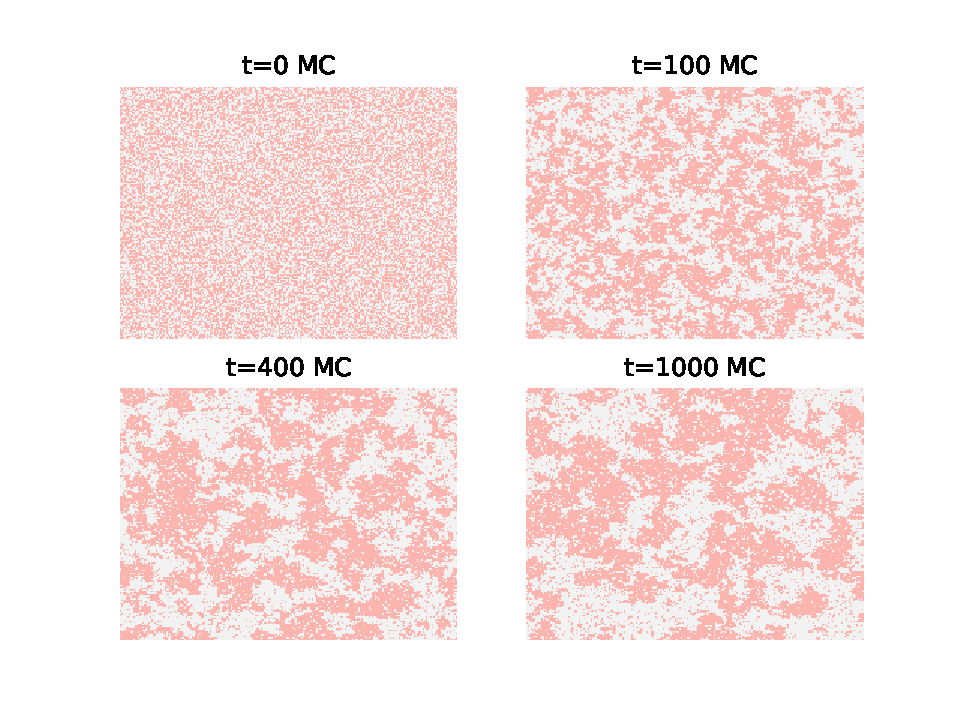
\includegraphics[width=\linewidth]{intro/clusterization.pdf}
    \caption{Numerical simulations of coarsening from a quench from a disordered state $T=\infty$ to an ordered state $T=T_{2D,C}$ \cite{onsager_crystal_1944} for different times, in Monte Carlo steps, for a $600 \times 600$ system with non-conserved Glauber dynamics.}
    \label{clusterization}
\end{figure}

While the phase diagram of a system can be determined via its Hamiltonian and equilibrium statistical mechanics, the dynamics of coarsening depends on the details of the systems dynamics that do not show up in single time thermodynamic observables. Therefore, one needs to construct dynamical models that capture the underlying evolution of the state of the system. In particular, there is a big difference between systems where the order parameter is conserved and those where it is not conserved.
%%%%%%%%%%%%%%%%%%%%%%
    \section{Models for equilibrium fields}
%%%%%%%%%%%%%%%%%%%%%%    

%%%%%%%%%%%%%%%%%%%%%%
    \subsection{Statics of systems with a finite number of degrees of freedom}
%%%%%%%%%%%%%%%%%%%%%%


Thermodynamic systems are naturally described in terms of fields, for example densities. 

Measuring observables in experimental setups means to measure the derivative of the partition function $Z$ with respect to its conjugate variable. This measure is done with a certain degree of spatial and temporal resolution, which means in a statistical language that they measure the average of the observable over some space and time. If $\Phi(\bx,t)$ is the physical field of our system, our device having a temporal resolution of $\Delta t$ and a spatial resolution over a volume $V$ will measure
\begin{align}
\phi(\bx,t) = \frac{1}{V \Delta t} \int_{t-\Delta t}^{t} dt' \int_V d\bx' \Phi(\bx',t')
\label{renormalisation}
\end{align}


This means that one is naturally lead to consider statistical field theories where the system is described in terms of a local field $\phi(\bx,t)$. Statistical field theories can be applied to both statics, to understand phase diagrams, and dynamics to understand phase ordering. However to start with we will examine the case of systems with a finite number of degrees of freedom. 

Consider a system in the canonical ensemble with a Hamiltonian $H(\bq)$ where $q_i$ for 
$1\leq i\leq N$ represent a finite number of continuous spatial degrees of freedom and where in a classical system we have already integrated over the corresponding momenta. The partition function for the system is given by
\begin{equation}
Z = \int d\bq \exp\left(-\beta H(\bq)\right)
\end{equation}
In general the integral which gives the partition function cannot be computed analytically. In equilibrium, the probability density function $P_{eq}(\bq)$ of the degrees of freedom is given by 
\begin{equation}
P_{eq}(\bq) = \frac{\exp\left(-\beta H(\bq)\right)}{Z}
\label{eqdis}
\end{equation}

The simplest approximation to compute $Z$ is the mean field approximation where the integral 
is approximated by the integrand at its largest value - in mathematics this is the Laplace method for approximating an integral and in this context it is just an expansion about the minimum energy configuration of the system. The mean field approximation is thus
\begin{equation}
Z_{MF}= \exp\left(-\beta H(\bq^*)\right)
\end{equation}
where $\bq^*$ is the value of $\bq$ which minimises $H$ (note that the approximation becomes exact in the zero temperature limit - $\beta \to \infty$ - as the system will minimise its energy). The values $q_i^*$ are determined from
\begin{equation}
\frac{\partial H}{\partial q_i}|_{\bq={\bf q^*}}=0
\end{equation}
Within this approximation any thermodynamic observable is given by
\begin{equation}
< f(\bq) > = f(\bq^*)
\end{equation}

We now consider how one can model dynamics of such systems. We will look for a Langevin equation which is chosen to give the correct equilibrium Gibbs-Boltzmann distribution. We write
\begin{equation}
\frac{d q_i}{dt} = -L_{ij}\frac{\partial H(\bq)}{ \partial q_j} + \eta_i(t)
\end{equation}
where $L_{ij}$ is a matrix which discuss later and $\eta_i(t)$ is zero mean Gaussian white noise with correlation function 
\begin{equation}
< \eta_i(t)\eta_j(t')> = \Gamma_{ij} \delta(t-t')
\label{cfn}
\end{equation}
The Gaussian white noise represents the effects of thermal fluctuations on the system we assume that the correlation time of these fluctuations is extremely short with respect to the dynamics of the degrees of freedom $q_i$ (in fact in critical systems the dynamics become very slow, critical slowing down, and this approximation becomes better and better as one approaches the critical point). There is no momentum term in this Langevin equation and for this reason it is often called the overdamped Langevin equation. Overdamped Langevin equations can also be derived staring from Newton's laws in the presence of friction, due to a solvent, and again white noise (again due to molecular collisions with the solvent) and by taking the limit where the frictional forces are greater than the acceleration term in Newton's equations (equivalent to setting the particle masses to zero).


As Eq. (\ref{cfn}) is for a correlation function the matrix $\Gamma_{ij}$ must be symmetric and cannot have any negative eigenvalues.

In the absence of noise or thermal fluctuations, so at zero temperature, the system will simply minimise its energy. Therefore if 
\begin{equation}
\frac{\partial H(\bq)}{ \partial q_j} =0
\end{equation}
with no noise we have $\frac{d q_i}{dt}=0$, that is to say it is the term $\frac{\partial H(\bq)}{ \partial q_j}$ that drives the dynamics if there is no noise. As long as the matrix $L_{ij}^{-1}$ exists the zero temperature dynamics will take the system to the local minimum of $H$ and to the absolute minimum if there are no metastable configurations. 


Under these assumptions, the Fokker-Planck equation for the probability density function of the degrees of freedom is 
\begin{equation}
\frac{\partial p(\bq,t)}{\partial t} = \frac{\partial}{\partial q_i} \left[\frac{1}{2}\Gamma_{ij} \frac{\partial p(\bq,t)}{\partial q_i} + p(\bq,t) L_{ij}\frac{\partial H(\bq)}{ \partial q_j}\right]
\end{equation}
This can be written as 
\begin{equation}
\frac{\partial p(\bq,t)}{\partial t} +\frac{\partial}{\partial q_i}J_i(\bq,t)=0
\end{equation}
where the ${\bf J}(\bq,t)$ is the probability current. We now insist that the system is in equilibrium with zero current when $p(\bq,t)= P_{eq}(\bq)$ as given by Eq. \eqref{eqdis}, this gives
\begin{equation}
\left[-\frac{\beta}{2}\Gamma_{ij} + L_{ij}\right]\frac{\partial H(\bq)}{ \partial q_j}
\end{equation}
and this holds for any choice of $H$ is we chose
\begin{equation}
\Gamma_{ij}= 2T L_{ij}
\end{equation}
where we have taken units where Boltzmann's constant $k_B=1$. 

%%%%%%%%%%%%%%%%%%%%%%
\subsection{Statistical field theory}
%%%%%%%%%%%%%%%%%%%%%%

We now consider a system with Hamiltonian $H[\phi]$ which depends on a continuous field $\phi(\bx)$. The partition function is given by a functional integral
\begin{equation}
Z = \int d[\phi] \exp(-\beta H[\phi]),
\end{equation}
the functional integral over all possible fields $\phi$ can be taken as a limit where $\phi$ is defined at a finite number of points on a lattice and then the lattice spacing is taken to zero. 
In many cases, the system has been coarse grained and $\phi$ represents a spatially varying order parameter, for instance the local density averaged over some small volume. In this case the Hamiltonian $H$ is strictly speaking a free energy and contains terms that depend on the temperature.

The mean field approximation to partition function is then given by
\begin{equation}
Z _{MF}= \exp(-\beta H[\phi_{MF}])
\end{equation} 
where $\phi_{MF}$ is the mean field solution which minimises $H$. The definition of a functional derivative of a functional is
\begin{equation}
F[\phi+\delta\phi]-F[\phi]= \int d\bx \frac{\delta F}{\delta\phi(\bx)} \delta\phi(\bx)
\end{equation}
Therefore if a field $\phi$ maximises $H$ we must have 
\begin{equation}
\frac{\delta H}{\delta\phi(\bx)}=0
\end{equation}

We now consider the standard Landau-Ginzburg Hamiltonian \cite{l_landau_physique_1990} describing Ising like systems where
\begin{equation}
H[\phi] = \int d\bx \ \frac{\kappa}{2}[\nabla \phi]^2 + V(\phi)
\label{landau-ginzburg-hamiltonian}
\end{equation}

The first term represents an energetic cost of varying the field $\phi$. The second potential term has two minima at $\phi=\pm \phi_c$, and, in the low temperature or phase separated phase, without loss of generality we can chose $V(\phi_c)=V(-\phi_c)$, while it has a single minimum at $\phi=0$ in the high temperature phase.

The standard potential for phase separations, called the $\phi^4$ model, is given by the double-well
\begin{align}
V(\phi) = \frac{1}{2} m^2 \phi^2 + \frac{\lambda}{4!} \phi^4
\label{phi4}
\end{align} 
where $m^2 = T-T_C$. For $m^2 \less 0$, the minima are at $\phi_C = \pm \sqrt{- \frac{6 m^2}{\lambda} } \pm$, while at $m^2 \ge 0$, the single minimum is at $\phi_C = 0$. We can also couple our system with the magnetic field of Hamiltonian
\begin{align}
H_1 &= - \int d^dx h(\bx)\phi(\bx)
\label{champ-externe}
\end{align}
As we in Fig \ref{double-puits-temperature}, the addition of an uniform external field does favour one phase over the other one.


\begin{figure}
\centering
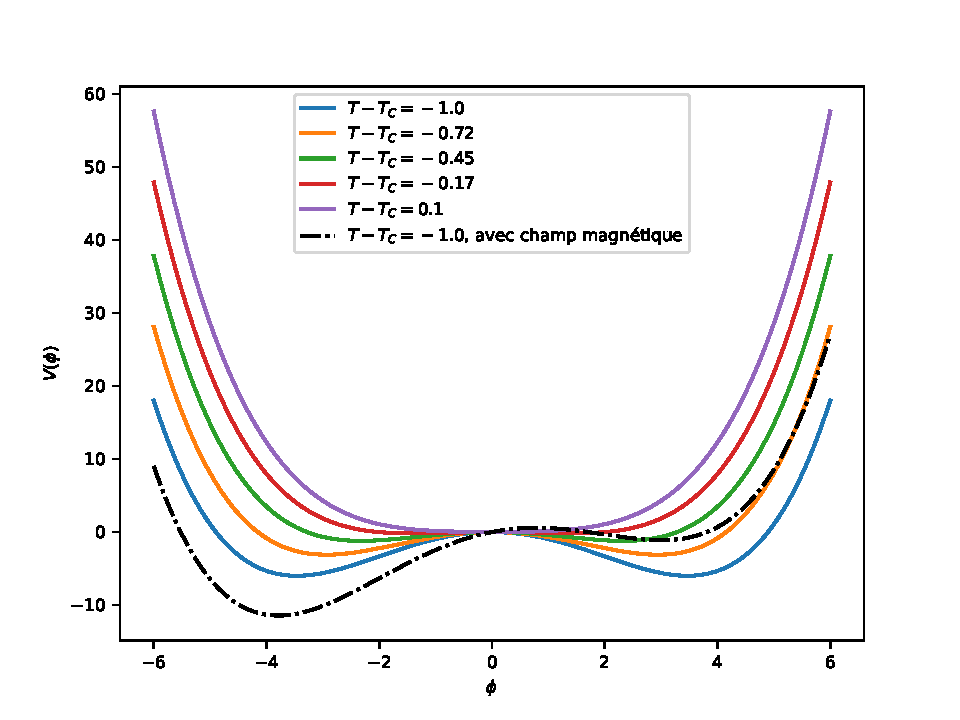
\includegraphics[width=0.6\linewidth]{intro/double-puit-en-fonction-temp.pdf}
\caption{Double-well potential \eqref{phi4} for $\lambda=1$ in function of the temperature difference with respect to the critical temperature with $m^2 = T-T_C$. In the ordered phase, the minima are at $\phi_C =\pm \sqrt{- \frac{6 m^2}{\lambda} } $, while for the ordered phase it is at $\phi_C = 0$. In black, the addition of a uniform magnetic field $h(\bx) = 1$ makes the positive phase metastable.}
\label{double-puits-temperature}
\end{figure}

It is easy to see that 
\begin{equation}
\frac{\delta H}{\delta \phi(\bx)} = -\kappa \nabla^2 \phi(\bx) + V'(\phi)
\label{cm}
\end{equation}
If we compare with systems with a discrete number of variables we
should have a Langevin equation of the form
\begin{equation}
\frac{\partial \phi(\bx)}{\partial t}= -L \frac{\delta H}{\delta \phi(\bx)} + \eta(\bx,t)
\end{equation}
The white noise correlator should have the form
\begin{equation}
< \eta(\bx,t)\eta(\bx',t)> =\delta(t-t')\Gamma(\bx,{\bf x'}),
\end{equation}
where here $\Gamma(\bx,{\bf x'})$ is an operator (before it was a matrix) defined by its action on functions $f$ as
\begin{equation}
\Gamma f(\bx) = \int d\bx' \Gamma(\bx,\bx')f(\bx')
\end{equation}
and $L$ is also an operator with 
\begin{equation}
L f(\bx) = \int d\bx' L(\bx,\bx')f(\bx')
\end{equation}
Following the same arguments for systems with a finite number of degrees of freedom we thus have the relation (which is sometimes called the fluctuation dissipation theorem as it essentially is equivalent)
\begin{equation} 
\Gamma(\bx,\bx') =2T L(\bx,\bx')
\label{gnoise}
\end{equation}

The simplest form of dynamics is given by $L(\bx,\bx')=\alpha\delta(\bx-\bx')$ which gives the \textbf{model A dynamics}
\begin{equation}
\frac{\partial \phi(\bx)}{\partial t}= -\alpha \frac{\delta H}{\delta \phi(\bx)} + \eta(\bx,t) 
\label{MA}
\end{equation}
with the noise correlator
\begin{equation}
< \eta(\bx,t)\eta(\bx',t)> =2T \alpha \delta(t-t')\delta(\bx-{\bf x'})
\end{equation}
The average value of $\phi$ 
\begin{equation}
\overline \phi(t) = \frac{1}{V}\int d\bx\ \phi(\bx,t)
\end{equation}
is clearly not generally conserved by this dynamics. Model A corresponds to a system in the grand-canonical ensemble, where $\alpha$ is the kinetic coefficient related to the relaxation time of the system \cite{hohenberg_theory_1977}.

\textbf{Model B dynamics} amounts to choosing
\begin{equation}
L(\bx-\bx')= -D\nabla^2 \delta(\bx-{\bf x'})
\end{equation}
The fact that $L$ is a positive semi-definite operator can be seen by taking its Fourier transform. The evolution equation here is
\begin{equation}
\frac{\partial \phi(\bx)}{\partial t}= D\nabla^2 \frac{\delta H}{\delta \phi(\bx)} + \eta(\bx,t)
\label{MB}
\end{equation}
where
\begin{equation}
< \eta(\bx,t)\eta(\bx',t)> =-2TD \delta(t-t')\nabla^2\delta(\bx-{\bf x'})
\end{equation}
We notice that if we introduce the vectorial white noise with components $\eta_i(\bx,t)$ such that
\begin{equation}
< \eta_i(\bx,t) \eta_i(\bx',t')> =\delta_{ij} \delta(\bx-{\bf x'})\delta(t-t)
\end{equation}
where $\delta_{ij}=1$ for $i=j$ and is zero otherwise, we can write
\begin{equation}
\eta(\bx,t)= \nabla\cdot {\boldsymbol \eta}(\bx,t)
\end{equation}
as one can verify the two noises have the same correlation function. In this way Eq. \eqref{MB} becomes 
\begin{equation}
\frac{\partial \phi(\bx)}{\partial t}= \nabla\cdot[ D\nabla \frac{\delta H}{\delta \phi(\bx)} + {\boldsymbol\eta}(\bx,t)]
\end{equation}
From this it is easy to see that the order parameter is conserved - thus model B describes conserved phase ordering dynamics. This model corresponds to the canonical ensemble, and is useful to describe diffusion or accretion systems.

Without the noise fluctuations, equations \eqref{MA} and \eqref{MB} are called the Time Dependant Ginzburg-Landau equation \cite{tuszynski_exact_1984} and the Cahn-Hilliard equation\cite{cahn_free_1958} equations, which give the mean field's dynamics.


%%%%%%%%%%%%%%%%%%%%%
\subsection{Surface tension}
%%%%%%%%%%%%%%%%%%%%%

In order to minimize the free energy in a non-conserved system, we can simply choose $\phi(\bx) =\phi_c$ or $\phi(\bx) =-\phi_c$ everywhere, which corresponds to a free energy $F=H[\phi_c]=0$. However in a system with a conserved order parameter
\begin{equation}
\int d\bx \ \phi(\bx)=0
\end{equation}
the solutions $\phi=\pm \phi_c$ cannot hold. In this case the system will separate into two homogeneous phases where $\phi(\bx)= \pm \phi_c$. We therefore choose an interface at $z=0$ and take $\phi(\bx) = \phi_K(z)$ ($K$ standing for kink as it is known as the kink solution in the literature) where $\lim_{z\to\-\infty}=-\phi_c$ and $\lim_{z\to\infty}=-\phi_c$. 
We therefore find from Eq. \eqref{cm} that
\begin{equation}
-\kappa \frac{d^2 }{dz^2}\phi_K(z) + V'(\phi_K) = 0 
\label{kk0}
\end{equation}
We can write
\begin{equation}
H[\phi_K]= A\int dz \ \frac{\kappa}{2}\left(\frac{d\phi_K(z)}{dz}\right)^2 + V(\phi_K(z))
\label{kk1}
\end{equation}
where $A$ is the surface area of the system in the plane perpendicular to the direction $z$. 
However, if we multiply Eq. \eqref{kk0} by $d\phi/dz$ and integrate we find
\begin{equation}
-\frac{\kappa}{2} (\frac{d\phi_K}{dz})^2 + V(\phi_K) = C
\end{equation}
where $C$ is a constant. However as $\phi_K(z)\to \pm \phi_c$ as $z\to \pm \infty$ and $V(\pm\phi_c) =0$ we find that $C=0$. Using this, we obtain 
\begin{equation}
H[\phi_K]= A\int dz\ {\kappa}\left(\frac{d\phi_K(z)}{dz}\right)^2 
\end{equation}
If the interface has a free energy per unit area of $\sigma$ then we have the Cahn-Hillard estimate of the surface tension \cite{cahn_free_1958}
\begin{equation}
\sigma= \int dz\ {\kappa}\left(\frac{d\phi_K(z)}{dz}\right)^2 
\label{CHST}
\end{equation}

In the case of the $\phi^4$ model defined at Eq \eqref{phi4}, the equation \eqref{kk0} becomes
\begin{align}
\kappa \phi_K''(z) = m^2 \phi_K(z) \left( 1 + \phi_C \phi_K(z) ^2 \right)
\label{eq-interface-glauber}
\end{align}
This potential is only defined by the ratio between $m^2$ and $\lambda$, so without loss of generality we set $\phi_C = 1$. The solution becomes
\begin{align}
\phi_K(z) = \tanh \left( \frac{z}{\xi} \right)
\label{profil-interface-glauber} 
\end{align}
where $\xi = \sqrt{\frac{-2 \kappa}{m^2}}$. This correlation length diverges when $T\to T_C$.
From Fig \ref{tension-xi} we see that the bigger the correlation length of the system, the smaller the surface tension is. The experimental study of quasi-critical systems, which have fluctuations at a macroscopic length scale, is a good way to probe the properties of ultra-low surface tension systems \cite{hennequin_drop_2006}. Such systems are very susceptible to hydrodynamic instabilities caused by thermal noise, as in microfluidics for example \cite{atencia_controlled_2005}. 
\begin{figure}
\centering
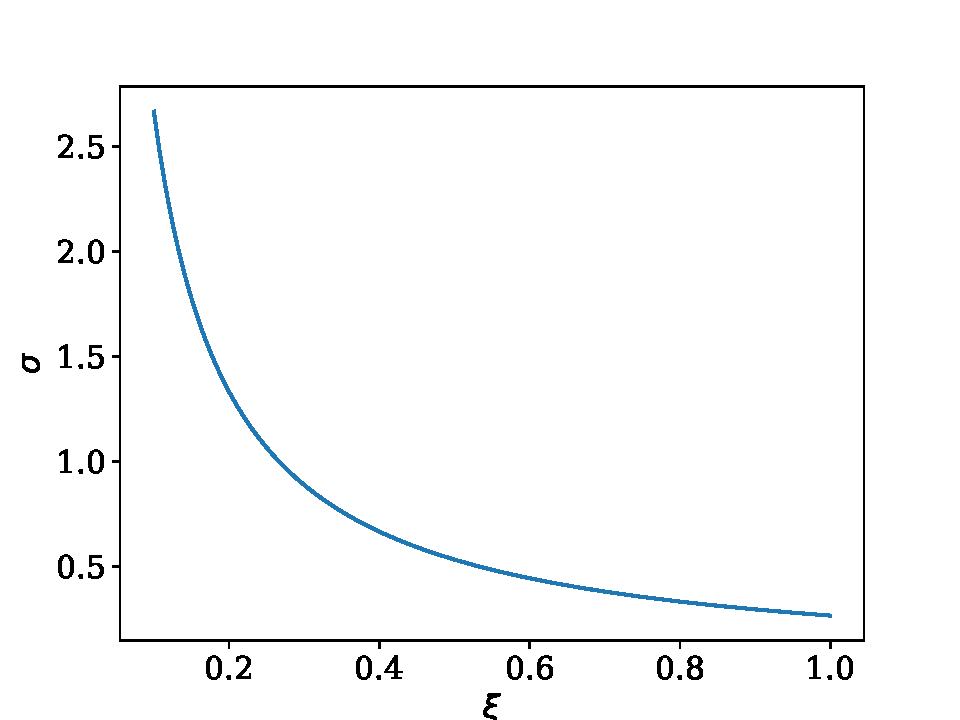
\includegraphics[width=0.7\linewidth]{int-dyn/tension-superficielle.pdf}
\caption{Surface tension \eqref{CHST} versus $\xi$ for the $\phi^4$ solution \eqref{profil-interface-glauber}.}
\label{tension-xi}
\end{figure}


%%%%%%%%%%%%%%%%%%%%%%
\section{Models for equilibrium interfaces}
\label{sec-continuous}
%%%%%%%%%%%%%%%%%%%%%%

%%%%%%%%%%%%%%%%%%%%%%
\subsection{Basic continuous model}
%%%%%%%%%%%%%%%%%%%%%%

Here we discuss effective models of interfaces. The simplest model is to assume that the 
interface is parameterised by a height profile $h(\br)$, where $\bx = (\br,z)$ however one also has to assume that 
$h(\br)$ is a single-valued function of $\br$. Given this one can write
\begin{equation}
H[h] = \sigma A[h]
\end{equation}
where $A[h]$ is the area of the interface. The interface area is given by
\begin{equation}
A[h] = \int_A d\br\sqrt{1+[\nabla h]^2}
\end{equation}
where the integral is over the plane perpendicular to the $z$ axis which is taken to be of area $A$. When the fluctuations of the interface are small, we can expand the above to quadratic order in $h$ to obtain
\begin{equation}
H[h]= A\sigma +\frac{\sigma}{2} \int_A d\br \ [\nabla h]^2
\end{equation}
The first term is independent of the height, so we can write the effective Hamiltonian for the surface as
\begin{equation}
H_{eff} [h]= \frac{\sigma}{2} \int_A d\br\ [\nabla h]^2
\label{heff}
\end{equation}

The basic model describing the height of an interface at $z=h(\br)$ above a plane with coordinates $\br$ has the Hamiltonian 
\begin{equation}
H[h] = \int d\bx\frac{\sigma}{2} [\nabla h(\bx)]^2 + V(h(\bx))
\end{equation}
The first term corresponds to the surface energy. In principle surfaces can also have bending energies, while surface energies correspond to stretching the surface to increase its size, bending energies correspond to curving the surface. The standard bending energy for small surface energies \cite{diehl_interface_1980} is given by
\begin{equation}
H_b[h] = \int d\br \frac{\kappa_b}{2}[\nabla^2 h(\br)]^2
\end{equation} 
where $\kappa_b$ is called the bending rigidity.

The term $V(h)$ is taken to represent the potential energy of the surface. For instance if the surface interacts via an infinite hard-core potential with a solid surface at $z=0$, this can be modelled by the potential $V(z) =0$ for $z \greater 0$ and $V(z)=\infty$ for $z\leq 0$. Another example is where the surface describes the surface of a liquid such as water, again with a solid surface at $z=0$, in the presence of gravity the potential energy of the water column above the area 
element $d\bx$ is given by
\begin{equation}
\delta V = \int_0^{h(\br)} dz\ \rho g z = \frac{1}{2}\rho g h^2(\br)
\end{equation}
where $\rho$ is the (mass) density of the liquid. This then gives
\begin{equation}
H[h] = \int d\br \frac{\sigma}{2}[\nabla h(\br)]^2 + \frac{1}{2}\rho g h^2(\br)
\end{equation}
We see that the correlation length of the interface is given by
\begin{equation}
\xi = \left(\frac{\sigma}{\rho g}\right)^{\frac{1}{2}}
\end{equation}
In the more general context, if $V(h)$ has a minimum at some point $h_m$ we can write $h= h_f(\bx)+ h_m$, where $h_f(\bx)$ represents the height fluctuations about the mechanically stable flat interface $h(\bx)=h_m$. Now expand assuming that $h_f(\bx)$ is
small we find the effective Hamiltonian for the fluctuations
\begin{equation}
H_{eff}[h_f] = \int d\br \frac{\sigma}{2}[\nabla h_f(\br)]^2 + \frac{1}{2}V''(h_m) h_f^2(\br)
\end{equation}
where we have dropped the constant term $AV(h_m)$. The above field theory is Gaussian and 
so, when the approximations made to derive it are valid, all of the statistical properties of the height fluctuations can be deduced. However for general potentials $V(h)$ the model cannot be solved exactly in two dimensions but can in principle be solved in one dimension as we will see below.

%%%%%%%%%%%%%%%%%%%%%%
\subsection{Effective dynamics of interface heights}
\label{sec-heightd}
%%%%%%%%%%%%%%%%%%%%%%
We will now try and derive an approximation for the dynamics of the height of the interface from the original phase ordering kinetics. Here we use the method of Bray and Cavagnha \cite{bray_interface_2001,bray_interface_2001-1}, which was used to study the dynamics of sheared interfaces, in the absence of shear to determine the dynamical properties of interfaces in phase separated systems for both model A and model B dynamics.

We imagine that the system is phase separated in the direction $z$, on average the interface is taken to be at $z=0$, and we write
\begin{equation}
\phi(z,\br,t) = f(z-h(\br,t))
\label{hans}
\end{equation}
where $f(z)=\phi_K(z)$ is the kink solution from mean field theory.

%%%%%%%%%%%%%%%%%%
\subsubsection{Model A dynamics}
%%%%%%%%%%%%%%%%%%

For model A dynamics, we substitute Eq. \eqref{hans} into Eq. \eqref{MA} and make use of the following results
\begin{align*}
\frac{\partial f(z-h(\br,t))}{\partial t} =& -f'(z-h(\br,t))\frac{\partial h(\br,t)}{\partial t}\\
\nabla f(z-h(\br,t) =& [{\bf e}_z-\nabla h(\br,t)]f'(z-h(\br,t)) \\
\nabla^2 f(z-h(\br,t))=& f''(z-h(\br,t))- \nabla^2 h(\br,t)f'(z-h(\br,t))+ [\nabla h(\br,t)]^2 f''(z-h(\br,t))
\end{align*}
and thus find
\begin{align*}
-f'(z-h(\br,t))\frac{\partial h(\br,t)}{\partial t}=& \alpha\kappa 
\left[ f''(z-h(\br,t))- \nabla^2 h(\br,t)f'(z-h(\br,t))+ [\nabla h(\br,t)]^2 f''(z-h(\br,t))\right] \\
& - \alpha V'(f'(z-h(\br,t))) + \eta(\br,z,t)
\end{align*}
We now multiply both sides of this equation by $f'(z-h(\br,t))$ and defining $\zeta=z-h(\br,t)$, we integrate $\zeta$ over $[-\infty,\infty]$ while using the following identities
\begin{align*}
\int_{-\infty}^\infty d\zeta f'(\zeta)f''(\zeta) =& [\frac{1}{2}f'^2(\zeta)]_{-\infty}^\infty =0 \\
\int_{-\infty}^\infty d\zeta f'(\zeta) V'(f) =& \int_{-\infty}^\infty d\zeta\frac{d V(f)}{d\zeta} =[V(f(\zeta))]_{-\infty}^\infty=0
\end{align*} 
Note that the first relation above holds as $f(\zeta)=\pm \phi_c$ as $\zeta\to\pm \infty$ and the second as
$V(\phi_c)=V(-\phi_c)=0$.
The terms that are left then give
\begin{equation}
-\int_{-\infty}^\infty f'^2(\zeta)d\zeta\ \frac{\partial h(\br,t)}{\partial t}
= -\alpha\int_{-\infty}^\infty f'^2(\zeta)d\zeta \ \kappa \nabla^2 h(\br,t) + \int_{-\infty}^\infty d\zeta \eta(\br,\zeta+ h(\br,t))f'(\zeta)
\end{equation}
Now using the Cahn-Hillard estimate of the surface tension, Eq. \eqref{CHST} thus becomes
\begin{equation}
\frac{\sigma}{\kappa} \frac{\partial h(\br,t)}{\partial t} = \alpha\sigma \nabla^2 h(\br,t) +\xi(\br,t)
\end{equation}
where the noise term is given by
\begin{equation}
\xi(\br,t)= -\int_{-\infty}^\infty d\zeta \eta(\br,\zeta+ h(\br,t))f'(\zeta)
\end{equation}
The noise term has zero mean and correlation function
\begin{align}
< \xi(\br,t)\xi(\br',t')> =&2\alpha T\delta(t-t')\delta(\br-\br')\int_{-\infty}^\infty d\zeta d\zeta' \delta(\zeta-\zeta')f'(\zeta)f'(\zeta')\nn
=& 2\alpha T\delta(t-t')\delta(\br-\br')\int_{-\infty}^\infty d\zeta f'^2(\zeta)= \frac{2\alpha T\sigma}{\kappa}\delta(t-t')\delta(\br-\br')
\end{align}
This now gives
\begin{equation}
\frac{\partial h(\br,t)}{\partial t}= \kappa\alpha \nabla^2 h(\br,t) + \eta(\br,t)
\end{equation}
where 
\begin{equation}
< \eta(\br,t)\eta(\br',t')> = \frac{2\alpha T\kappa}{\sigma}\delta(t-t')\delta(\br-\br')
\end{equation}
Now defining $\alpha' = \frac{\kappa\alpha}{\sigma}$ we can write
\begin{equation}
\frac{\partial h(\br,t)}{\partial t}= \alpha' \sigma\nabla^2 h(\br,t) + \eta(\br,t)
\end{equation}
This has the form of model $A$ dynamics (as in Eq. \eqref{MA}) for the height profile with Hamiltonian
$H_{eff}$ as given in \eqref{heff}, that is to say we can write
\begin{equation}
\frac{\partial h(\br,t)}{\partial t}= -\alpha' \frac{\delta H_{eff}[h]}{\delta h(\br)} + \eta(\br,t)
\label{ew}
\end{equation}
with
\begin{equation}
< \eta(\br,t)\eta(\br',t')>= 2T\alpha'\delta(t-t')
\end{equation}
This dynamical calculation is thus consistent with the idea of describing the surface in terms of a height variable with an energy given by the surface tension. The equation \eqref{ew} is known as the Edwards-Wilkinson equation \cite{edwards_surface_1982,halpin-healy_kinetic_1995}. We can use this equation to determine how the domains of a coarsening system grow at low temperatures. To do this we ignore the noise term and assume that at $t=0$ the correlations of the height are short range. so
\begin{equation}
C(\br-\br',0)= < h(\br,0)h(\br',0)> =C_0 \delta(\br-\br')
\end{equation}
In Fourier space the noiseless Edwards-Wilkinson equation becomes
\begin{equation}
\frac{\partial\tilde h(\bk,t)}{\partial t} = -\alpha'\sigma k^2\tilde h(\bk,t) 
\end{equation}
and so we find
\begin{equation}
\tilde h(\bk,t) = h(\bk,0)\exp(-\alpha'\sigma\bk^2 t)
\end{equation}
The two point correlation function becomes
\begin{equation}
< \tilde h(\bk,t)\tilde h(\bk',t')> = < h(\bk,0)h(\bk',0)> \exp(- \alpha'\sigma[k^2+k'^2] t).
\end{equation}
Now recall that if 
\begin{equation}
< h(\br,t) h(\br',t')> =C(\br-\br',t)
\end{equation}
then
\begin{equation}
< \tilde h(\bk,t)\tilde h(\bk',t')>= (2\pi)^d \delta(\bk+\bk') \tilde C(\bk,t)
\end{equation}
where 
\begin{equation}
\tilde C(\bk,t)= \int d\br \exp(-i\bk\cdot \br)C(\br,t)
\end{equation}
is the Fourier transform of the correlation function, which is a function of a single position due to invariance by translation in space, and $d$ is the dimension of space (so here $d=2$ for a surface in 3d space and $d=1$ for a surface in a 2d space). Putting all this together gives
\begin{equation}
\tilde C(\bk,t)= C_0 \exp(-2\alpha'\sigma k^2 t)
\end{equation}
Inverting the Fourier transform, we have
\begin{equation}
C(\br,t)= \frac{C_0}{(8\pi \alpha'\sigma t)^{\frac{d}{2}}} \exp(-\frac{\br^2}{16\pi \alpha'\sigma t})
\end{equation}
From this we see that if $C(\br,t)\sim g(\frac{\br}{\ell(t)})r(t)$ then the length scale $\ell(t)\sim t^{\frac{1}{2}}$, this agrees with what is found in the Ising model under Glauber dynamics, where the growth exponent is also given by $z=\frac{1}{2}$\cite{paul_domain_2005}.

%%%%%%%%%%%%%%%
\subsubsection{Model B dynamics}
%%%%%%%%%%%%%%

For model B dynamics, we take the same ansatz as in Eq. \eqref{hans} but we rewrite the model B dynamics as
\begin{equation}
-\nabla^{-2} \frac{\partial\phi(\bx,t)}{\partial t} = -D \frac{\delta H}{\delta \phi(\bx)}+ \theta(\bx,t)
\end{equation}
here $-\nabla^{-2}$ represents the Green's function $G$ which obeys 
\begin{equation}
\nabla^2 G(\bx-{\bf x'}) = -\delta(\bx-\bx')
\end{equation}
and 
\begin{equation}
\theta(\bx,t)=-\nabla^{-2}\eta(\bx,t)= \int d\bx'G(\bx-{\bf x'})\eta(\bx,t)
\end{equation}
The correlation function of $\theta(\bx,t)$ is given by
\begin{align}
< \theta(\bx,t)\theta({\bf y},t')> =&-2DT\delta(t-t') \int d\bx'G(\bx-{\bf x'})d{\bf y}'G({\bf y}-{\bf y'})\nabla^2\delta(\bx'-{\bf y}') \nn
=& -2DT\delta(t-t') \int d\bx'G(\bx-{\bf x'})d{\bf y}'\nabla^2G({\bf y}-{\bf y'})\delta(\bx'-{\bf y}') \nn
=& 2DT\delta(t-t') G(\bx-{\bf y})
\end{align}
where we have integrated by parts in the second line and used 
\begin{equation}
-\nabla^2G({\bf y}-{\bf y'})= \delta({\bf y}-{\bf y}')
\end{equation}
in the third.

Now multiplying by $f'(z-h(\br,t))$ and integrating $z$ over $[-\infty,\infty]$, we find
\begin{align}
-\int dz f'(z-h(\br,t))\int dz'd\br'\ G(z-z',\br-\br') f'(z'-h(\br',t))\frac{\partial h(\br',t)}{\partial t} = -D\sigma \nabla^2 h(\br,t) + \chi(\br,t),
\end{align}
with the noise
\begin{equation}
\chi(\br,t)= \int dz f'(z-h(\br,t)) \theta(\br,z,t).
\end{equation}
As we assume that the height fluctuations are small, we keep only the lowest order terms in $h$ in the deterministic terms and the noise, we will see later that this is compatible thermodynamically. We thus have
\begin{equation}
-\int dz \ f'(z)\int dz'd\br'\ G(z-z',\br-\br') f'(z')\frac{\partial h(\br',t)}{\partial t} = -D\sigma \nabla^2 h(\br,t) + \chi(\br,t)
\end{equation}
and now the noise is given by
\begin{equation}
\chi(\br,t)= \int dz\ f'(z) \theta(\br,z',t)
\end{equation}
This equation which is linear in $h$ can now be Fourier transformed in the plane $\br$. In terms of the Fourier transform of $h$ we find
\begin{equation}
-\int dz \ f'(z)\int dz'd\br'\ \tilde G(z-z',\bk) f'(z')\frac{\partial\tilde h(\bk,t)}{\partial t} = Dk^2\sigma \tilde h(\bk,t) + \tilde \chi(\bk,t)
\label{bstep}
\end{equation}
The Fourier transform of $G$ in the $\br$ plane obeys
\begin{equation}
\frac{d^2 \tilde G(z-z',\bk )}{dz^2}-k^2 \tilde G(z-z',\bk )=-\delta(z-z')
\end{equation}
and the solution to this equation (with the boundary condition that $\tilde G(z-z',\bk )\to 0$ as $|z-z'|\to\infty$) is
\begin{equation}
\tilde G(z-z',\bk) = \frac{\exp(-k|z-z'|)}{2k}
\end{equation}
where we have used the notation $k=|\bk|$, so $k$ is positive. Next we make the sharp interface approximation where we write
\begin{equation}
f(z) = 2\phi_c \delta(z)
\label{sharp}
\end{equation}
that is to say we have replaced the smooth kink solution with a step like solution
$f(z) = \phi_c\ {\rm sgn}(z)$. This then gives
\begin{equation}
-4\phi_c^2 \tilde G(0,k) \frac{\partial h(\bk,t)}{\partial t} = Dk^2\sigma \tilde h(\bk,t) + \tilde \chi(\bk,t)
\end{equation}
which we rewrite as
\begin{equation}
\frac{\partial \tilde h(\bk,t)}{\partial t} = -\frac{Dk^3\sigma}{2\phi_c^2} \tilde h(\bk,t) + \tilde \xi(\bk,t)
\end{equation}
with 
\begin{equation}
\tilde \xi(\bk,t)= - \frac{k}{2\phi_c^2}\tilde \chi(\bk,t)
\end{equation}
where 
\begin{equation}
\tilde \chi(\bk,t)= \int dz\ f'(z) \tilde\theta(\bk,z,t)
\end{equation}
The correlation function of $\tilde \theta(\bk,t)$ is 
\begin{equation}
< \theta(\bk,t)\theta(\bk',t')> = 2DT(2\pi)^d \delta(t-t') \delta(\bk+{\bf k'}) \tilde G(z-z',k)
\end{equation}
From this we find 
\begin{equation}
< \chi(\bk,t)\chi(\bk',t')> = 2DT(2\pi)^d \delta(t-t') \delta(\bk+{\bf k'}) \int dz dz' f(z) f(z') \tilde G(z-z',k)
\label{bstep2}
\end{equation}
Now, using the sharp interface approximation Eq. \eqref{sharp}, we obtain
\begin{equation}
< \chi(\bk,t)\chi(\bk',t')> = 2DT(2\pi)^d \delta(t-t') \delta(\bk+{\bf k'}) \frac{2\phi_c^2}{k}
\end{equation}
and consequently
\begin{equation}
< \xi(\bk,t)\xi(\bk',t')> = 2DT(2\pi)^d \delta(t-t') \delta(\bk+{\bf k'}) \frac{k}{ 2\phi_c^2}
\end{equation}
Finally in we find the interface dynamics for model B in Fourier space is
\begin{equation}
\frac{\partial h(\bk,t)}{\partial t} = -\frac{Dk^3\sigma}{2\phi_c^2} \tilde h(\bk,t) + \tilde \xi(\bk,t)
\label{modBFT}
\end{equation}
In real space this has the form
\begin{equation}
\frac{\partial h(\br)}{\partial t}= -L \frac{\delta H_{eff}}{\delta h (\br)} + \xi(\br,t)
\end{equation}
where the operator $L$ is defined via its Fourier transform
\begin{equation}
\tilde L(\bk) = \frac{Dk}{2\phi_c^2}
\end{equation}
Now if we look at Eq. \eqref{modBFT} we see that solving the equation without noise will give a function of $k^3t$, which in real space corresponds to $x^3/t$. From this we see that the coarsening length scale grows as $\ell(t) \sim t^{\frac{1}{3}}$ and consequently the coarsening exponent is $z=\frac{1}{3}$. Coarsening for conserved model B or diffusive dynamics is slower than that of model A \cite{huse_corrections_1986}. One of the reasons for this slowing down with respect to nonconserved dynamics is that material must be physically transported by diffusion (by exchanging spins in the language of lattice spin models), where as for model A dynamics the composition can change at any given point by {\em spin flipping}. As a cautionary note, if we had taken the Hamiltonian in Eq. \eqref{heff} and applied model B conserved dynamics, as in Eq. \eqref{MB}, for the height field we would not have obtained this equation. 

We can actually do better than the above sharp interface approximation as Eq. \eqref{bstep} can be written as
\begin{equation}
Q(k)\frac{\partial\tilde h(\bk,t)}{\partial t} = -Dk^2\sigma \tilde h(\bk,t) - \tilde \chi(\bk,t)
\label{bstep2}
\end{equation}
where 
\begin{equation}
Q(k)= \int dzdz' \ f'(z)\ \tilde G(z-z',\bk) f'(z')
\end{equation}
Notice that from Eq. \eqref{bstep2} that
\begin{equation}
< \chi(\bk,t)\chi(\bk',t')> = 2DT(2\pi)^d \delta(t-t') \delta(\bk+{\bf k'}) Q(k)\end{equation}
and so 
\begin{equation}
\frac{\partial\tilde h(\bk,t)}{\partial t}= -\tilde L(k) \tilde \mu(\bk) + \eta(\bk)
\end{equation}
where $\mu(\bx)=\delta H_{eff}/\delta h(\bx) $, $\tilde L(k) = D/Q(k)$ and 
\begin{equation}
< \eta(\bk,t)\eta(\bk',t')> = 2T(2\pi)^d \delta(t-t') \delta(\bk+{\bf k'}) \tilde L(k)
\end{equation}

%%%%%%%%%%%%%%%%%%%
    \section{Lattice models}
%%%%%%%%%%%%%%%%%%%

%%%%%%%%%%%%%%%%%%%%%%%%%%%%%%%%%%%%%%%%%%%%%
    \subsection{The Ising model}
%%%%%%%%%%%%%%%%%%%%%%%%%%%%%%%%%%%%%%%%%%%%%  


We take a system of size $L'\times L' \times L$, composed of $N$ sites $i$. At each site corresponds a value $\sigma_i =\pm1$. The Hamiltonian of the Ising model is 
\begin{equation}
	H =  - \sum_{<ij>} J \sigma_i \sigma_j + \frac{V(\sigma_i)+V(\sigma_j)}{2}
	\label{hamil-ising}
\end{equation}
where $\sum_{< ij >}$ is a sum over all pairs of nearest neighbours, and the external field $V(\sigma_i)$ has been symmetrized. The Ising model\cite{niss_history_2005,niss_history_2009} is therefore a lattice model with short interactions between particles. Since all particles $\sigma_i$ in the system are equal to $\pm!$, this system is called a lattice based spin model. When $\sigma_i$ is continuous, it is called the XY model \cite{gupta_phase_1988}.
$J$ is called the coupling parameter of the system, and can be non-uniform, with the nearest neighbours interaction being $J = J_{ij}$. If $ J_{ij} =0$, the system favorises homogeneous phases and is called ferromagnetic. Otherwise, the system favorises configurations where each spin has an opposite sign with respect to all of their neighbours, which modelises antiferromagnetic materials. We will pose $J=1$.

\begin{figure}[t]
	\begin{minipage}[t]{0.5\linewidth}
		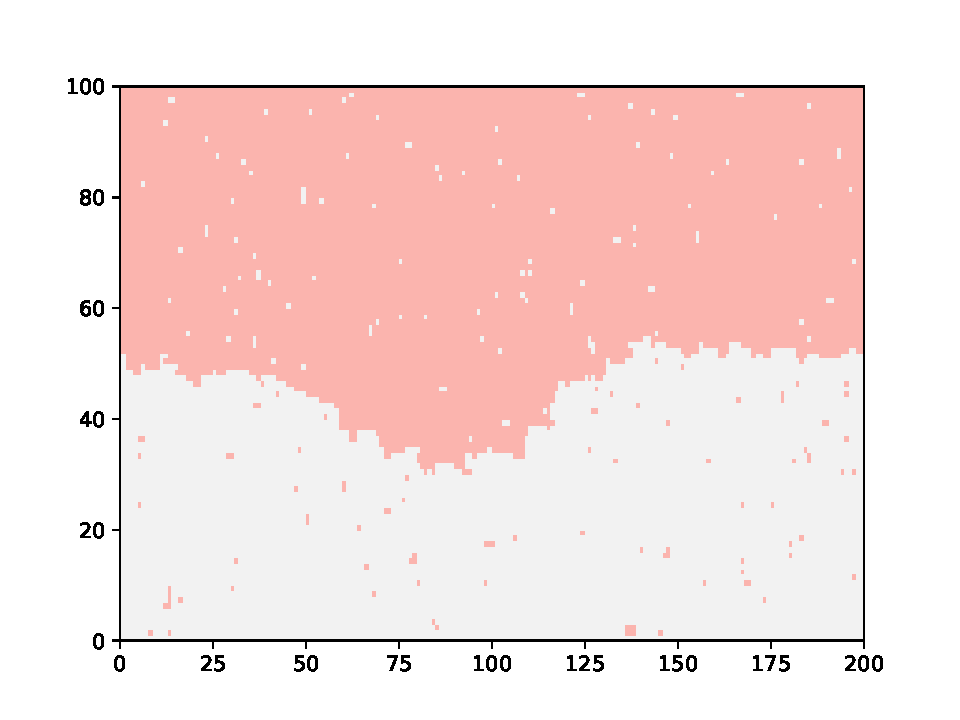
\includegraphics[width=\linewidth]{int-dyn/inte07.pdf}
	\end{minipage}%
	\begin{minipage}[t]{0.5\linewidth}
		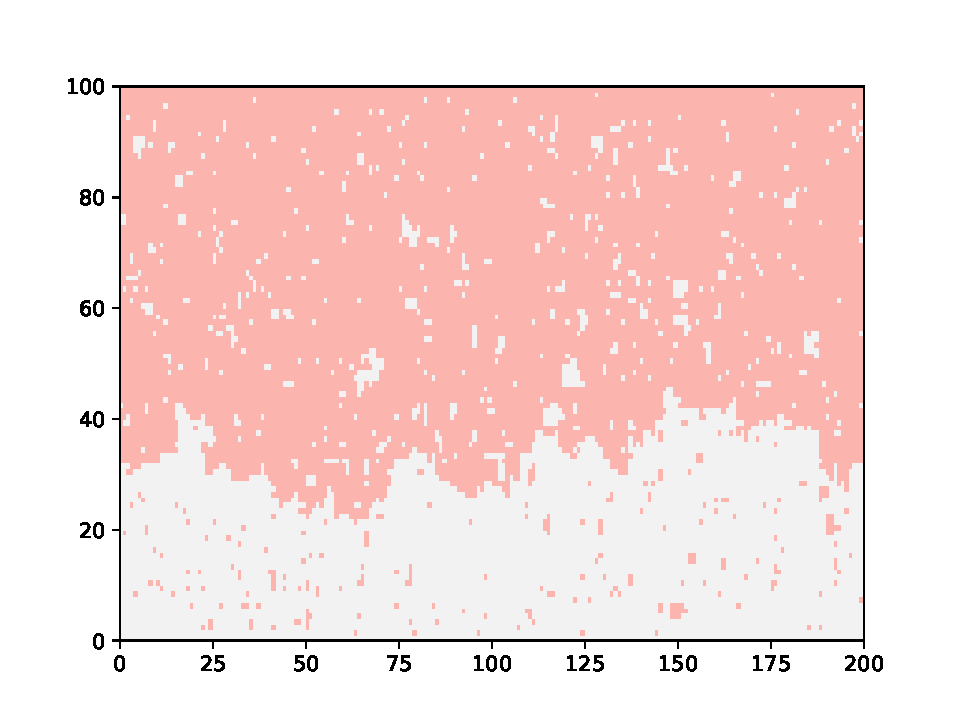
\includegraphics[width=\linewidth]{int-dyn/inte09.pdf}
	\end{minipage}
	\caption{Snapshot of Monte Carlo simulations of the Ising model for two different temperatures in two dimensions($T=0.7 T_C$ (left) and $T=0.95 T_C$ (right)) with periodic boundary conditions in $x$ and fixed ones in$y$.}
	\label{amas-fixe}
\end{figure}  


The mean-field theory with a $\phi^4$ potential has been developed from this model \cite{bellac_equilibrium_2004}. Exact relationship between both of them has been found in 4 dimensions and above \cite{aizenman_proof_1981}. A fast way to convince ourselves is to take the finite difference derivative at first order of Eq \eqref{landau-ginzburg-hamiltonian}. If we suppose the sole role of the potential is to set the field to $\pm \phi_C$ on each site, then we have
\begin{align}
    [{\boldsymbol \nabla} \phi(i)]^2 &= \left( \frac{\partial \phi(i)}{\partial x} \right)^2  + \left( \frac{\partial \phi(i)}{\partial y} \right)^2 + \left( \frac{\partial \phi({\bf i})}{\partial z} \right)^2\nn
    &= (\phi(x,y,z)-\phi(x+1,y,z))^2 + (\phi(x,y,z)-\phi(x,y+1,z))^2 + (\phi(x,y,z)-\phi(x,y,z+1))^2 \nn
    &= 2 (1-\phi(x,y,z)\phi(x+1,y,z) + 2 (1-\phi(x,y,z)\phi(x,y+1,z) +2 (1-\phi(x,y,z)\phi(x,y,z+1) 
    \label{discretisation-landau}
\end{align}
where we've set the distance between two sites to $1$.
From this we easily see some bulk energy to which we add the sites' nearest neighbours interactions in an Ising-like fashion.
%%%%%%%%%%%%%

This model precisely describes  phase transitions in uniaxial magnetic systems\cite{de_jongh_experiments_1974,wp_wold_ising_2000,ikeda_neutron_1973}. It is also the simplest model of its eponymous universality class, which also contains liquid/gas transitions and binary fluids.
In these mappings, $n_i=\frac{1}{2}(1-\sigma_i)=0,1$ represents occupation of a cell of a lattice fluid or $\sigma_i$ gives the label of a binary species $A$ or $B$.
This model does not have a phase transition in 1D, but a phase transition in 2D was foumd in 1944\cite{onsager_crystal_1944} at the critical temperature 
\begin{align}
     T_{2D,C} = \frac{2J}{k_B \ln(1 + \sqrt{2})} \simeq 2.27 \frac{J}{k_B}
\end{align}

The renormalization group approaches have a deep connexion with the Ising model \cite{frohlich_triviality_1981,goldenfeld_lectures_2018}. Even though results have been found for $d=4$ (which is the upper critical dimension), no analytical solution has been found in 3 dimensions. Numerous numerical simulations  \cite{talapov_magnetization_1996,preis_gpu_2009} have shown that the 3-dimensional phase transition occurs at 
\begin{align}
    T_{3D,C} \simeq 4.51 \frac{J}{k_B}
\end{align}


By making the transformation\cite{goldenfeld_lectures_2018} 
\begin{align}
    n_i =  \frac{\sigma_i +1}{2}
\end{align}
so that $n_i(\sigma_i = 1) = 1$ and $n_i(\sigma_i = -1) = 0$, we obtain
\begin{equation}
	H =  - \sum_{< i j >}  J_{ij} \left( 4 n_i n_j -2 ( n_i+n_j) + 1 \right)+ \sum_{< i j >}  \frac{V(\sigma_i)+V(\sigma_j)}{2}  
\end{equation}
where the constant term $\sum_{< i j >}  J_{ij}$ does not change the partition function behaviour. We have then
\begin{align}
	H_{LG} &=  - 4 \sum_{< i j >}  J_{ij}  n_i n_j  + 2 \sum_{< i j >}  J_{ij}  (n_i+n_j) + \sum_{< i j >}  \frac{V(\sigma_i)+V(\sigma_j)}{2}  \nn
       &=  - 4 J \sum_{< i j >}  J n_i n_j  + \mu \sum_i  n_i + \sum_{< i j >}   \frac{V(\sigma_i)+V(\sigma_j)}{2}  
\end{align}
where we have set $J_{ij} = J$ constant and defined the intrinsic chemical potential for a liquid-gas system as $\mu_c=4J c$, with  $c$ the number of nearest neighbours. A positive magnetic phase is thus analogous to a high density state such a liquid, while the negative magnetic phase is equal to a low density state such as a gas. An onsite potential $V(\sigma_i)$ further modifies the chemical potential, $\mu=\mu_c+\delta\mu[V(\sigma_i)]$.
The chemical potential $\mu$ is the conjugate variable to the total number of particles $\sum_i n_i$, while the magnetic field $B$ is the conjugate variable to the total magnetisation $\sum_i \sigma_i$. The two are connected through the mapping such that $B\sim \mu-\mu_c$, so that liquid-gas and Ising model systems share common thermodynamic features such as the universality class for critical fluctuations. For the fluid the grand canonical ensemble corresponds to the Gibbs ensemble with fixed $T$ and $\mu$ and canonical ensemble with fixed $T$ and $N$ . In the magnetic system these ensembles correspond to fixed $T, B$ and $T,M$ respectively. The model also describes adsorption of a gas in a lattice or binary fluids between particles of different species $A$ and $B$.



By imposing $+-$ boundary conditions in the $z$ direction, we force the existence of an interface Those BC can be fixed, imposing  $\sigma(z=0) = -1$ and $\sigma(z=L)=+1$, or free but with a local external field $V(z) = h (\delta_{0,z}-\delta_{z,L})$.
An interface is characterized by its mean and its width. The easiest way to do so is to fit the magnetization profile
\begin{align}
    m(z) = \frac{1}{L'^2} < \sum_{xy} \sigma(x,y,z) >
\end{align}
to mean field results from Eq \eqref{profil-interface-glauber} . The mean position of the interface is
\begin{align}
    m = <h> = \frac{1}{L'^2} < \sum_i \sigma_i >
\end{align}
The width of the interface is then defined  as 
\begin{align}
    w^2 = <h^2>-<h>^2
\end{align}
This can be rewrtiten \cite{stecki_magnetization_1994} as
\begin{align}
    w^2 = 2 \frac{ \int_0^L dz z \frac{d m(z)}{dz}}{\int_0^L dz \frac{d m(z)}{dz}}
\end{align}
We now defined the surface tension of the interface as the free energy difference between  the bulk and interface \cite{richards_numerical_1993}. Is $Z^{++}$ si the partition function of a system with $(++)$ BC, and $Z^{+-}$ with $(+-)$ BC, then the surface tension \cite{abraham_interface_1976} is given by
\begin{align}
    \sigma &= \lim_{L',L \to \infty} \frac{1}{L'^2} \ln \left( \frac{Z^{+-}}{Z^{++}} \right) 
\end{align}
By diagonalization of the transfer matrix (which we will define later), we find that the surface tension of a the interface between two pure phases $+$ and $-$ is given in a two-dimensional Ising model \cite{abraham_transfer_1973} by
\begin{align}
    \sigma = 2 \beta J + \log(\tanh(\beta J))    
\end{align}

%%%%%%%%%%%%%%%%%%%%%%%%%%%%%%%	
\newpage	
    \subsection{The Solid-On-Solid Model}
    \label{sec-sos}
%%%%%%%%%%%%%%%%%%%%%%%%%%%%%%%  


In order to get the Edwards-Wilkinson equation of an interface from statistical field theory, we have used the approximation 
\begin{align}
\phi(\bx,t) = f(z-h(\br,t))
\end{align}
We translate the same approximation in order to study interfaces in lattice models by
\begin{align}
\sigma_{i,j} = \sgn(h_i-j)
\label{approx-sos}
\end{align}
where $\sgn(x \less 0) = -1$ and $\sgn(x \greater 0) = 1$, and $h_i$ is the height of the interface at site $i$. 
This is the low temperature approximation of the Ising model, where there are no overhangs from the $+$ phase into the $-$ phase and vice versa. If we note $J_\perp$ the vertical bond energy between two Ising spins and $J_\parallel$ the horizontal bond energy, this approximation becomes equivalent to a highly anisotropic Ising model where $J_\perp \gg J_\parallel$ \cite{swendsen_roughening_1977}.

In a slab or semi-infinite geometry as seen in Fig \ref{figure-sos}, the height of the interface corresponds to the number of spins $-$ in the column $i$, while for an infinite geometry, we define $h_i$ as the number of excess spins $-$ with respect to the mean height, set in the figure at $=0$ \cite{van_leeuwen_pinning_1981}. In this representation, height profiles represent an interface height and not a number of particles, since there is no entropy term associated with the number of ways that the $h_i$ particles on each site can be chosen from the $N$ particles available. In chapter \ref{chap-pop}, we will address a model with those characteristics.
Using the identities
\begin{align}
\min(a,b) &= \frac{|a+b| - |a-b|}{2} \\
\max(a,b) &= \frac{|a+b| + |a-b|}{2}
\end{align}
we have
\begin{align}
\sum_{j=0}^L \sgn(h-j)\sgn(h'-j) = L - 2 |h-h'|
\end{align}
For a 2-D Ising model of size $L'\times L$, the Ising Hamiltonian \eqref{hamil-ising} is rewrtiten as
\begin{align}
H = 2 J L' (1-L) +2 J \sum_{i=0}^{L'} |h_i-h_{i+1}| + \sum_{i=0}^{L'} V(h_i)
\label{energie-sos-ising}
\end{align}
with external potential 
\begin{align}
V(h_i) = \sum_{j=0}^L V(\sgn(h_i-j))
\end{align}
For periodic boundary conditions, we set $h_{L'}=h_0$.

\begin{figure}
    \begin{minipage}[t]{0.5\linewidth}
        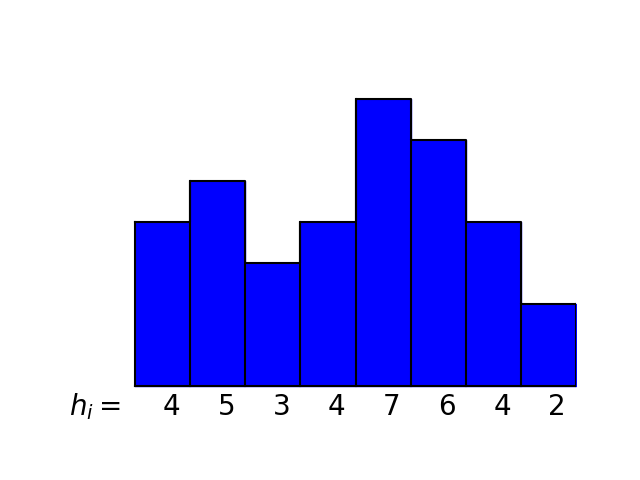
\includegraphics[width=0.9\linewidth]{int-dyn/sos-indiscernable.png}
    \end{minipage}
    \begin{minipage}[t]{0.5\linewidth}
        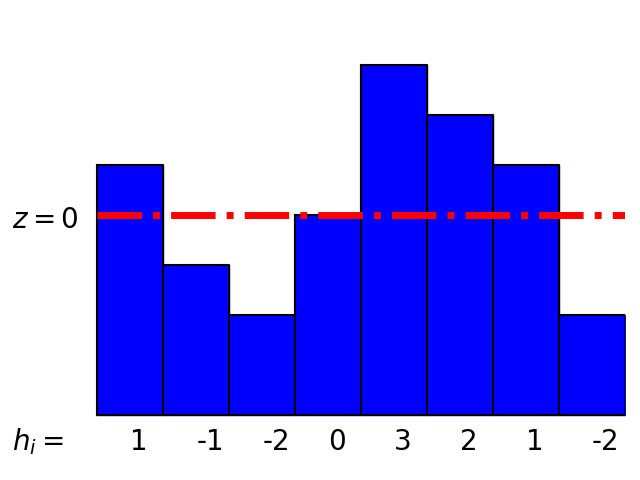
\includegraphics[width=0.9\linewidth]{int-dyn/sos-indiscernable-inf.png}        
    \end{minipage}    
    \caption{Possible configuration of the SOS model for a semi-infinite geometry (left) and infinite geometry (right). The red line shows the origin $z=0$. In the $i$-th column the interface is at height $h_i$. Particles under the interface are from the Ising $-$ phase, while particles over it are from the $+$ phase.}
    \label{figure-sos}
\end{figure}

Another way to compute this energy for a SOS configuration is to directly count the number of energy bonds for a $L'\times L$ Ising model under the approximation \eqref{approx-sos}. There are $L-1$ vertical bonds per column, where all have an energy of $-J$, while the link that goes though the interface has an energy of $+J$. The total contribution to energy from vertical bonds is thus 
\begin{equation}
    E_\perp = - J L' ( L-2)
\end{equation}
There are $L'\times L$ horizontal bonds. In a pure phase system, the horizontal energy would be $-JL'L$. Neverthelesss, there are $\sum_i |h_i-h_{i+1}|$ bonds which have an energy of $+J$, which gives the horizontal energy  contribution 
\begin{equation}
    E_\parallel = - J L' L + 2 \sum_i |h_i-h_{i+1}|
\end{equation}
By adding both, we find back Eq \eqref{energie-sos-ising}.

By setting $2J=J$ and getting rid of the bulk energy, we obtain the \textbf{Solid-On-Solid Hamiltonian} 
\begin{align}
H = J \sum_{i=0}^{L'} |h_i-h_{i+1}| + \frac{V(h_i)+V(h_{i+1})}{2}
\label{hamil-sos}
\end{align}



The first system where the SOS model has been applied was crystals' growth in 1972 \cite{gilmer_simulation_1972}. Since then, the model has been used with some success in naphthalene cristals\cite{elwenspoek_kinetic_1987}, experimental expitaxial growth\cite{wilby_scaling_1992}, polymer membranes \cite{boal_mechanics_nodate,gompper_steric_1989}, or interfacial wetting \cite{fisher_walks_1983}.

In the SOS model, the sites $i$ of height $h_i$ can take any value in $[0,L]$. The Restrictied Solid-On-Solid model (RSOS) is a variation where sites can only take the value $h_{i+1} \in [h_i-1,h_i,h_i+1]$\cite{privman_transfer-matrix_1989}. This approximation works for very low temperatures or very smooth interfaces \cite{kim_conserved_1994,vaysburd_critical_1995}. 

Another model, closer to the continuous model of Hamiltonian \eqref{heff} is the Discrete Gaussian model which has the following gaussian interaction
\begin{align}
H = J \sum_{i=0}^{L'} (h_i-h_{i+1})^2 + \frac{V(h_i)+V(h_{i+1})}{2}
\label{hamil-gsos}
\end{align} 
and also has a restricted version. The SOS model has an exact relation with the $XY$ model \cite{knops_exact_1977}, no matter the power law used for the interaction. With a generalization of this model to continuous heights, it has been shown that extreme deviations statistics of the interface is described by a scaling function \cite{schehr_universal_2006}. Since the energy costs of height differences $0,\pm 1$ are the same in every SOS model no matter the exponent  in the energy costs of height differences, one expects the qualitative freatures of all those models to be the same at low temperature, since height differences are typically small \cite{swendsen_monte_1977}.



Since the dimensionality of the system has been reduced in only taking into account the height interface $h_i$ at site $i$ instead of the position of all particles, we can think of an interface as a partially self-avoiding walk. This idea, which will be developed in section \ref{sec-continuous-model}, has proven quiet powerfull in finding exact solutions of the generating function \cite{owczarek_exact_1993} or the extreme deviations statistics of the interface \cite{majumdar_airy_2005,schehr_universal_2006}.

In the canonical ensemble, the height interface is fixed to $N$, which is translated in the partition function as
\begin{align}
Z(N) = \sum_{h_0 h_1 ... h_{L'}} \exp(- \beta \sum_{i} H(h_i,h_{i+1})) \delta_{\sum_i h_i, N}
\label{hamil-sos-cano}
\end{align}
In the grand-canonical ensemble, the conjugate variable to the height interface is the chemical potential $\mu$, and the grand partition function $\Xi$ is related to the canonical partition function by
\begin{align}
\Xi(\mu) =& \sum_N Z(N) \exp((\beta \mu N) \nn
=& \sum_{h_0 h_1 ... h_{L'}} \exp(-\beta H_{eff}(h_0,h_1,...,h_{L'})
\label{hamilk-sos-gce}
\end{align}
where
\begin{align}
H_{eff} = J \sum_{i=0}^{L'} |h_i-h_{i+1}|+ \sum_{i=0}^{L'} V(h_i)-\mu h_i
\end{align}
In Fig \ref{hauteur-mu}, we plot the mean number of particles per site with respect to the chemical potential, for different size of the system, in the thermodynamic limit $L' \to \infty$. When the chemical potential is too small, the Lagrange's multiplier of the mean height is negligible, allowing the interface to fluctuate freely. Since the height of the interface is then evenly spread over all possible configurations, the mean value for $\mu=0$ becomes $\frac{L}{2}$.


\begin{figure}
\centering
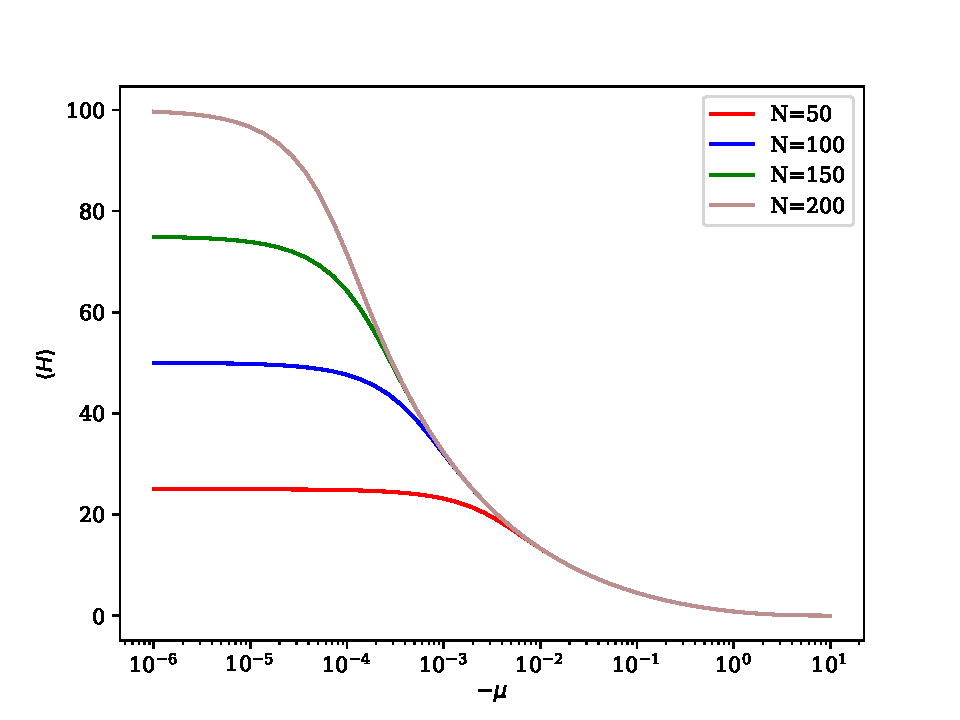
\includegraphics[width=0.7\linewidth]{int-dyn/hauteur-tm-sos.pdf}
\caption{Mean height of the SOS interface \eqref{hamilk-sos-gce} with respect to $- \mu$ through diagonalization of the transfer matrix for $\beta=1$, in the limit $L'\to \infty$. }
\label{hauteur-mu}
\end{figure}

%%%%%%%%%%%%%%%%%%%%%%%%%%%%%%%%%%%%%%%
\subsection{Transfer matrix}
%%%%%%%%%%%%%%%%%%%%%%%%%%%%%%%%%%%%%%%


In a more general fashion, we can rewrite the Hamiltonian as
\begin{align*}
H = \sum_{i=0}^{L'} f(h_i,h_{i+1}) + V(h_i,h_{i+1}) 
\end{align*}
where $f(h_i,h_j)$ is the energy interaction between two nearest neighbours and $V(h_i,h_j)=\frac{V(h_i)+V(h_j)}{2}$ is the external potential. We can rewrite the partition function as 
\begin{align}
Z = \sum_{h_1=0}^{L} \sum_{h_2=0}^{L}... \sum_{h_{L'}=0}^{L} \exp(- \beta \sum_{i=0}^{L'} H(h_i,h_{i+1}))
= \sum_{h_1 h_2 ... h_{L'}} \prod_{i=_0}^{L'} \exp(-\beta H(h_i,h_{i+1}))
\end{align}
We define the transfer matrix
\begin{align}
T(h_i,h_j) = e^{-\beta H(h_i,h_j)}
\label{matric-transfert}
\end{align}
In Fig \ref{mat-inf}, we have represented an infinite matrix corresponding the limit $L\to \infty$, where each site can take any value in $[-\infty,\infty]$. To diagonalize numerically such matrices, we translate the whole system with $h_i \to h_i - \frac{L}{2}$, where $L$ is the matrix's size, which me make tend to $\infty$.
The constraint \eqref{hamil-sos-cano} cannot be expressed in the transfer matrix formalism, which induces a change in properties from this ensemble with respect to the transfer matric results \cite{siegert_scaling_1993}.

Since the system has periodic boundary conditions $h_{L+1} = h_1$, we have $T(h_L,h_{L+1}) = T(h_L,h_1)$ \cite{pearce_exact_1989}. The matrix is thus symmetric, which means it can be diagonalized with eigenvectors and eigenvalues 
\begin{align}
T | \lambda> = \lambda |\lambda>
\end{align}
Those eigenvectors are orthonormal
\begin{align}
< \lambda | \lambda'> = \delta_{\lambda \lambda'}
\end{align}
We set $\lambda_0$ as the biggest eigenvalue of $T$, by $\lambda_1$ the second biggest eigenvalue, and so on. The partition function can then be rewritten, in terms of the transfer matrix \cite{abraham_transfer_1973} by
\begin{align}
Z = \sum_{h_1 h_2 ... h_{L'}} \prod_{i} T(h_i,h_{i+i}) = Tr( T^{L'}) = \sum_\lambda <\lambda | T^{L'} | \lambda> = \sum_\lambda \lambda^{L'}
\label{partition-trace-lambda}
\end{align}

\begin{figure}
\begin{align}
T = \begin{bmatrix} 
\ddots & \vdots & \reflectbox{$\ddots$} \\ 
e^{-\beta H(-1,-1)} & e^{-\beta H(-1,0)} & e^{-\beta H(1,-1)} \\
\dots & e^{-\beta H(0,0)} & \dots \\
e^{-\beta H(1,-1)} & e^{-\beta H(1,0)} & e^{-\beta H(1,1)} \\ 
\reflectbox{$\ddots$} & \vdots &\ddots \\ 
\end{bmatrix}
\end{align}
\caption{Infinite and symmetrical transfer matrix \ref{matric-transfert}.}
\label{mat-inf}
\end{figure}

In the thermodynamic limit $L' \to \infty$, only the biggest eigenvector is relevant since the partition function becomes
\begin{align}
Z(L\to \infty) \simeq \lambda_0^{L'}
\end{align}
We find that the free energy per site is 
\begin{align}
f = - \frac{1}{L' \beta} \ln(Z) \simeq - \frac{1}{\beta } \ln( \lambda_0)
\label{energie-libre-site}
\end{align}
In Fig \ref{fig-thermo-libre} we plot the evolution of the free energy per site $\Omega(L')$ without external field, compared to the thermodynamic limit. We determine that the thermodynamic limit becomes valid for $L' \greater 150 $.

\begin{figure}
\centering
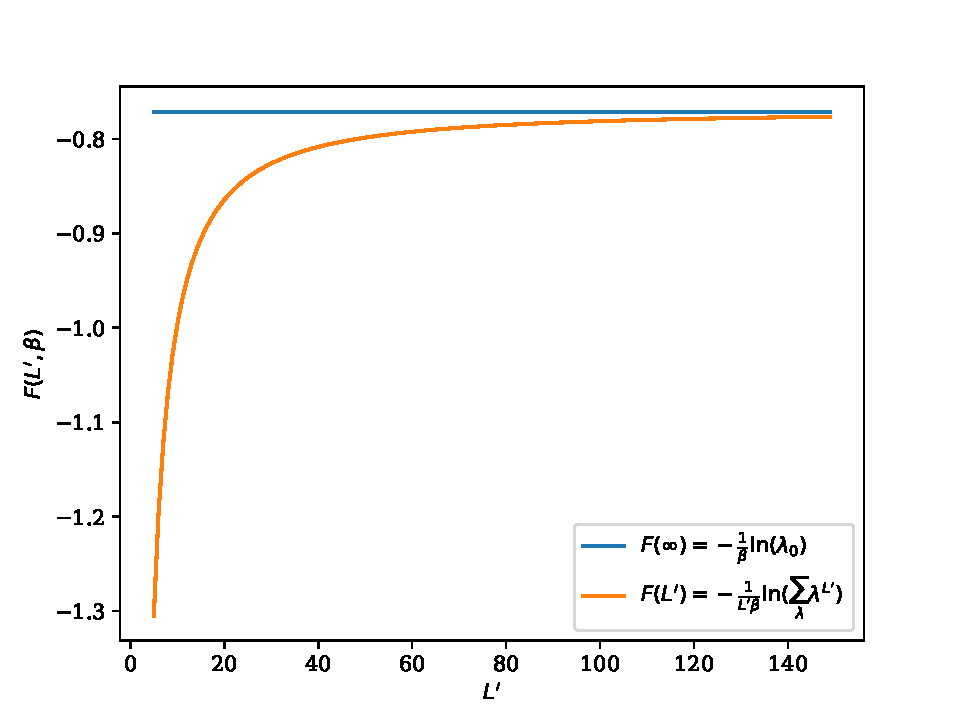
\includegraphics[width=0.7\linewidth]{int-dyn/freeene-thermo-libre.pdf}
\caption{Free energy per site $\Omega(L')$ with respect to the number of sites $L'$ compared to the thermodynamic value $\Omega(\infty)$, for a system of maximum height $L=100$, $\beta=1$, $J=1$ and $V(h_i)=0$.}
\label{fig-thermo-libre}
\vspace{-0.5cm}
\end{figure} 

To compute the mean height value per site $M$, we introduce the height matrix $\hat{M}$ defined by its action over the vectors $|h>$ in the matrix transfer's base by
\begin{align}
= \delta_{h,h'} h
\end{align}
We thus find that the density is
\begin{align}
M = < h > = \frac{1}{L'} \sum_i h_i = \frac{1}{Z} \sum_\lambda \lambda^{L'} < \lambda | \hat{M} | \lambda > \simeq < \lambda_0 | \hat{M} | \lambda_0 > 
\label{tm-magnetisation}
\end{align}
We deduce the mean displacement per site
\begin{align}
w^2 = < (h - M)^2 > = \frac{1}{Z} \sum_\lambda \lambda^{L'} < \lambda | \hat{M}^2 | \lambda > - < \lambda | \hat{M}| \lambda >^2 \simeq < \lambda_0 | \hat{M}^2 | \lambda_0 > - M^2
\end{align}
We can find thos two obersables by computing the first and second moment of the probability distribution that a site $i$ is at height $h_i$
\begin{align}
p(h) = \frac{1}{Z} \sum_\lambda \lambda^{L'} <\lambda | h >^2 \simeq < \lambda_0 | h >^2
\end{align}
The two-point correlation function of the system is computed by
\begin{align}
C(r) &= < h_i h_{i+r} > - M^2 = \frac{1}{Z} \sum_{\lambda \neq \lambda_0} < \lambda_0 | M | \lambda > < \lambda | M | \lambda_0 > \left( \frac{\lambda}{\lambda_0} \right)^r 
\end{align}
which becomes, in the long distance $r$ limit, 
\begin{align}
C(r) \simeq < \lambda_0 | M | \lambda_1 > < \lambda_1 | M | \lambda_0 > \left( \frac{\lambda_1}{\lambda_0} \right)^r
\end{align}
The correlation function has an exponential decay at large distances, which allows us to define the correlation length at large distance $\xi$
\begin{align}
\xi = - \frac{1}{\ln(\frac{\lambda_1}{\lambda_0})}
\label{longueur-correl-thermo}
\end{align}

%
%%%%%%%%%%%%%%%%%%%%%%%%%%%%%%%%%%%%%%
%	\subsection{États libres dans un système SOS infini}
%	\label{par-stab}
%%%%%%%%%%%%%%%%%%%%%%%%%%%%%%%%%%%%%%
%
%Prenons un système de taille $L$ dans la limite thermodynamique $L'\to \infty$. Comme vu précédement, seules les valeurs de la plus grand valeur propre influe sur les propriétés statistiques. Soit 
%\begin{align}
%    \psi_\lambda(h)= <h|\lambda>
%\end{align}
%la projection du vecteur propre associé à la valeur propre $\lambda$ de la matrice de transfert sur la base des hauteurs $|h>$ dans un système infini de part et d'autre de l'interface.
%Dans la limite $\beta=0$, c'est-à-dire pour une température infinie, tous les termes de la matrice de transfert sont égaux à $1$, menant à des vecteurs propres nuls. Dans ce cas, la densité de probabilité $p(h)$ est nulle pour tout $h$, ce qui signifie qu'il n'existe pas d'interface. Le modèle SOS n'est donc pas valable dans cette limite. De même, pour une température nulle $\beta=\infty$, la matrice de transfert devient la matrice identité. Les valeurs propres deviennent toutes égales à $1$ et les vecteurs propres sont $\psi_i(h) = \delta_{h,i}$ où ici $i$ est l'indice de la i-ème valeur propre $\lambda_i = 1$. La probabilité de trouver l'interface à la hauteur $h$ devient $p(h) = \frac{1}{Z}\sum_{i} <\lambda_i | h >^2 = 1$. La température nulle a pour effet de geler l'interface sur une seule hauteur, même si toutes les hauteurs sont équiprobables. Bien que les micro-états soient extrêmement différents pour une température finie, les propriétés macroscopiques sont identiques à cause du même poids statistique associé à chaque état.
%
%Pour une température finie et en absence de potentiel\cite{guyer_sine-gordon_1979,chui_pinning_1981}, l'équation du vecteur propre donne
%\begin{align}
%	\sum_{h=-\infty}^\infty T(h,h') \psi_\lambda(h) = \lambda \psi_\lambda(h')
%\end{align}
%En introduisant l'ansatz $\psi_\lambda(h) = \alpha_{\lambda}^h$ et en séparant de la somme les termes pour $h$ négatifs et positifs, on trouve aisément que 
%\begin{align}
%	\lambda = \frac{\sinh(\beta J)}{\cosh(\beta J)-(\alpha_{\lambda}+\alpha_{\lambda}^{-1})} 
%\end{align}
%Dans la limite thermodynamique, la probabilité de présence de l'interface à la hauteur $h$ est $p(h) = <\lambda_0|h>^2 = |\psi_0(h)|^2$. Le système ne possédant aucune brisure de symétrie particulière, la probabilité $p(h)$ est finie pour tout $h$ avec $p(h)=p(-h)$. Dès lors, l'ansatz supposé $\psi_\lambda(h) = \alpha_{\lambda}^h$ implique que $\alpha_{\lambda}$ soit de la forme $e^{ik}$ où $k$ est la longueur d'onde associée à la valeur propre $\lambda$. On obtient que 
%\begin{align}
%	\psi_k(h) =& e^{ikh} \\
%	\lambda =& \frac{\sinh(\beta J)}{\cosh(\beta J) - \cos(k)}
%	\label{lambda-sos}
%\end{align}
%
%L'existence d'une solution de ce genre indique que l'interface n'est pas localisée dans le cas d'un système infini (ou semi-infini) en absence de tout potentiel, ce qui conduit à de nombreux problèmes numériques. 
%
%Une manière simple de localiser l'interface est de rajouter un potentiel $V(h) = -B \delta_{h,0}$ \cite{chui_pinning_1999,chalker_pinning_1981,chalker_pinning_1982}, qui augmente la probabilité de présence de l'interface à $h=0$. La recherche d'un état localisé nous donne un ansatz de la forme 
%\begin{align}
%	\psi_\lambda(h) = \begin{cases} |\alpha|^h & \text{si } h \neq 0 \\ \psi_{\lambda,0} & \text{sinon} \end{cases} 
%\end{align}
%L'équation du vecteur propre devient
%\begin{align}
%	\sum_{h=-\infty}^\infty \exp(\beta |h-h'|- \beta B \delta_{h,0}) \psi_\lambda(h) = \lambda \psi_\lambda(h')
%\end{align}
%En notant $T(h,h') = R^{|h-h'|}$ pour $h \neq h' \neq 0$,  on obtient la même équation à un signe près dans l'exposant que l'on soit à $h'\greater 0$ ou $h' \greater 0$
%\begin{align}
%	\left( \frac{R}{\alpha} \right)^{\pm h'} \left[ \psi_{\lambda,0} + \frac{R \alpha}{1 - R \alpha} + \frac{\alpha}{R - \alpha} \right] + \left[ \frac{1}{1-R \alpha} - \frac{R}{R-\alpha} \right] = \lambda
%\end{align}
%Puisque cette équation est vraie pour tout $h'$, le premier terme doit être nul, ce qui nous donne
%\begin{align}
%	\psi_{\lambda,0} &= - \frac{\alpha}{R-\alpha}-\frac{R \alpha}{1-R \alpha} \\
%	\lambda &= \frac{1}{1-R \alpha} - \frac{R}{R-\alpha}
%\end{align}
%L'équation du vecteur propre à $h'=0$ nous donne par ailleurs 
%\begin{align}
%	\psi_{\lambda,0} + 2 \frac{R \alpha}{1-R \alpha} = \lambda \psi_{\lambda,0} e^{-\beta B}
%\end{align}
%L'existence d'une solution cohérente $\alpha \less 1$ autorise la présence d'une interface localisée grâce à un potentiel dit d'épinglage (\textit{pinning}) \cite{burkhardt_localisation-delocalisation_1981,kroll_solid--solid_1981,kroll_pinning_1982,kroll_interface_1983}.
%Dans le cas d'une géométrie semi-infinie, la présence d'un potentiel chimique exerçant une pression sur l'interface permet de la maintenir confinée, comme expliqué dans la section \ref{subsec-c-gc}.
%
%D'autres méthodes existent pour confiner l'interface. Le cisaillement d'une interface diminue sa largeur et permet de la localiser dans l'espace. On peut également proposer deux potentiels chimiques différents pour chaque phase à une hauteur de l'interface prédéfinie, comme le ferait un laser dans un liquie binaire dont chaque phase  a un incident de réfraction différent \cite{casner_laser-induced_2003,delville_laser_2009} (voir chapitre \ref{sec_laser}). Dans un système infini, une autre possibilité est de définir un champ magnétique symétrique rendant plus difficile la présence de l'interface loin de $0$. 


%%%%%%%%%%%%%%%%%%%%%%
    \section{Systems driven by imposed hydrodynamic flows}
%%%%%%%%%%%%%%%%%%%%%%

\begin{figure}
\centering
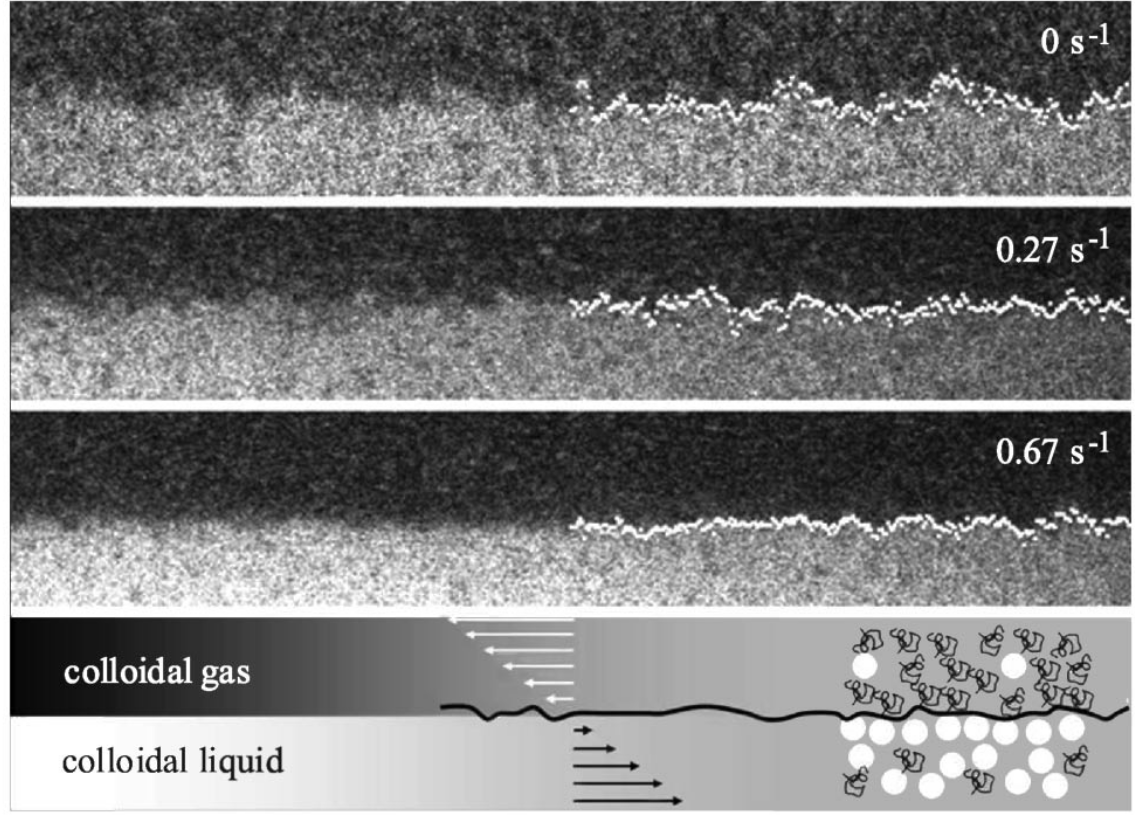
\includegraphics[width=0.7\linewidth]{int-dyn/derks.png}
\caption{Snapshot of the interface a sample of fluorescently labeled poly(methyl methacry-late) (PMMA) colloidal spheres in polystyrene close to the critical point, for different shear rates. The bottom panel schematically shows the flow geometry with the plane of zero velocity located at the interface. From \cite{derks_suppression_2006}. }
\label{snap-derks-shear}
\vspace*{\floatsep}
\begin{minipage}[t]{0.5\linewidth}
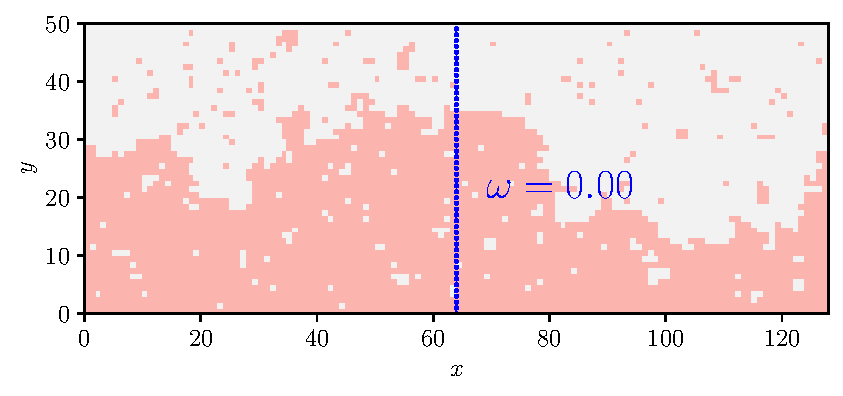
\includegraphics[width=\linewidth]{intro/cis-ising-f-000.pdf}
\end{minipage}%
\begin{minipage}[t]{0.5\linewidth}
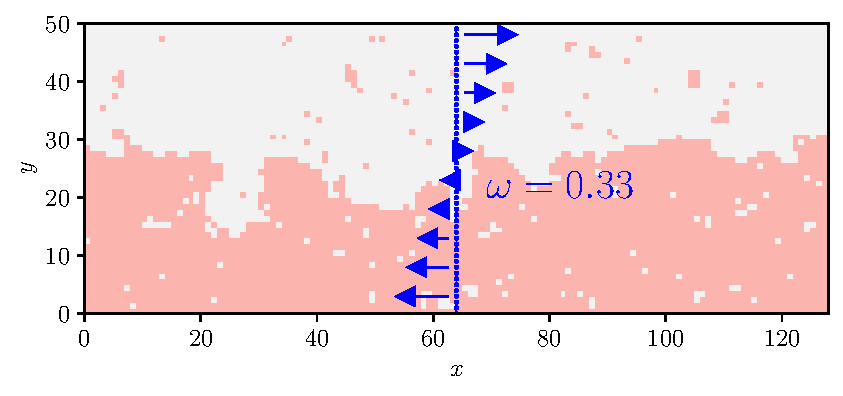
\includegraphics[width=\linewidth]{intro/cis-ising-f-033.pdf}
\end{minipage}
\centering
\begin{minipage}[t]{0.5\linewidth}
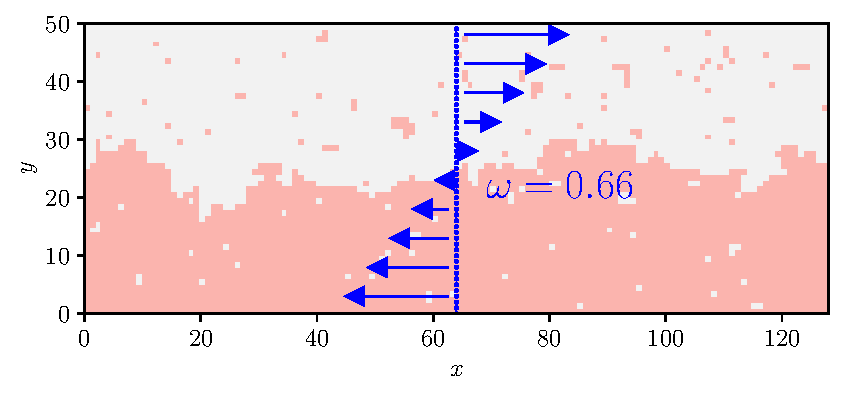
\includegraphics[width=\linewidth]{intro/cis-ising-f-066.pdf}
\end{minipage}
\caption{Snapshot of a 2D Ising model with respect to the shear \eqref{eq-cisaillement} with Kawasaki dynamics at $T=0.9 T_{2D,C}$.}
\label{snap-ising-shear} 
\end{figure} 

Here we consider what happens when a system is driven out of equilibrium. By driven we mean that energy is injected into the system by a laser \cite{girot_conical_2019}, by inducing a hydrodynamics flow, for instance a shear flow induced in a Couette cell in liquids \cite{derks_confocal_2004,derks_suppression_2006} or in glassy materials \cite{berthier_nonequilibrium_2002,berthier_shearing_2002}. In principle we should analyse this system with model H dynamics which couples diffusive model B dynamics to hydrodynamics in the low Reynolds number Stokes flow regime. In these dynamics the order parameter field will itself induce a hydrodynamics flow which will modify
the imposed one. However this full situation is very difficult to analyse and to a first approximation we can assume that the back reaction of the order parameter field on the hydrodynamic flow is small with respect to the imposed hydrodynamic flow and so we can simply write
\begin{equation}
\frac{\partial \phi (\bx,t)}{\partial t} + \nabla\cdot({\bf v}(\bx)\phi(\bx,t)) =- L\frac{\delta H}{\delta \phi(\bx)} + \eta(\bx,t),
\label{drive}
\end{equation}
where $L$ is given by the underlying model A or B dynamical operator and the noise has the correlation function as given by Eq. \eqref{gnoise}, and ${\bf v}(\bx)$ is the imposed (time independent) hydrodynamic flow or can equally well be an external drive imposed on the colloidal particles, due to the gravitational or electric field for example. 

The simplest case one can consider is where the driving field ${\bf v}(\bx) ={\bf v}_0$ is uniform \cite{leung_field_1986.bray_coarsening_2000}. Unfortunately this simple driving does not lead to a new steady state. Basically all of the colloidal particles acquire an average velocity ${\bf v_0}$ and so move along at the same speed relative to each other. Mathematically this can be seen by making the Galilean transformation
\begin{equation}
\phi (\bx,t)= \phi(\bx-{\bf v}_0t,t) = \phi({\bf y},t)
\end{equation}
This transformation eliminates the driving from the evolution equation \eqref{drive} and so we find an equilibrium system. 

The most studied example is where the driving is a shear flow \cite{derks_suppression_2006,thiebaud_nonequilibrium_2010}. The effective dynamics of the surface term in the presence of a shear flow, parallel to the interface \cite{bray_interface_2001,bray_interface_2001-1,}, is written as
\begin{equation}
{\bf v}(\bx) = \gamma z {\bf e}_x
\label{eq-cisaillement}
\end{equation}
and was studied using the method explained in section (\ref{heightd}). The addition of a shear flow leads to the appearance of a nonlinear term in $h$ and the interface statistics thus become non-Gaussian. In Fig \ref{snap-ising-shear} we show the influence of such a shear flow in numerical simulations, which is exactly the behaviour to be seen in capillary waves in polymer melts \cite{derks_confocal_2004,derks_suppression_2006}, see Fig \ref{snap-derks-shear} . The shear has a confining effect on the interface \cite{smith_driven_2010,smith_interfaces_2008-1,smith_interfaces_2008}, thus increasing the effective surface tension of the system.




%%%%%%%%%%%%%%%%%%%%
\section{Conclusion}
%%%%%%%%%%%%%%%%%%%% 

Statistical field theory \cite{bray_theory_1994} gives us a method to study the dynamics of equilibrium fields \cite{bellac_equilibrium_2004}. The surface tension of such a system is then defined as the difference of free energy between the bulk and the interface \cite{cahn_free_1958,abraham_transfer_1973}. The two main models are model A and model B \cite{hohenberg_theory_1977}, which decribe the dynamics of a field respectively in grand-canonical and the canonical ensemble. From those equations, we have defined what is an interface and have derived the Edwards-Wilkinson equation \cite{edwards_surface_1982} for both ensembles.
The Ising model \cite{niss_history_2005,niss_history_2006} provides a good way to study the bahviour of the field by discretization, which is easier to compute in numerical simulations \cite{newman_monte_1999}. The same kind of dimensional reduction can be done in order to get an interface lattice model which is called the Solid-On-Solid model \cite{gilmer_simulation_1972}. This model allows the use of the transfer method in an easier way than the Ising model\cite{privman_asymptotic_1989}. 
Also, the presence of out-of-equilibrum hydrodynamic flows tend to present interesting features. One such example is thee Couette shear \cite{derks_suppression_2006}, which has been found to smoothen the interface \cite{smith_interfaces_2008-1}.
